\documentclass{beamer}

\usepackage[utf8]{inputenc}
\usepackage{algorithm}
\usepackage{algpseudocode}

\usetheme[%
    numbering=fraction,
    progressbar=foot,
]{metropolis}

\setbeamercolor{frametitle}{use=normal text}


\title{Parallelization of the Mean Shift Clustering with OpenMP}
\author{Emilio Cecchini}
\institute{
    Università degli Studi di Firenze \\
    \medskip
    \textit{emilio.cecchini@stud.unfi.it}
}
\date{\today}


\begin{document}


\maketitle


\begin{frame}{Overview}
\tableofcontents
\end{frame}


\section{The Mean Shift Clustering}

\begin{frame}{Mean Shift key concepts}

\begin{itemize}
\item
Non-parametric technique to find the maxima of a density function.
\item
At each step, a \textit{kernel function} is applied to each point that causes the points to shift in the direction of the local maxima determined by the kernel.
\end{itemize}

\end{frame}


\begin{frame}{Gaussian Kernel}

\begin{itemize}
\item
There are many different types of kernel, the most used is the \textit{Gaussian kernel}:

\begin{align*}
k(x) =  e^{-\dfrac{x}{2\sigma^2}}
\end{align*}
\item
The standard deviation $\sigma$ is the bandwidth parameter, with a high bandwith value you will get a few large clusters and vice versa.
\end{itemize}

\end{frame}


\begin{frame}{Mean Shift Clustering}
Suppose $x$ is a point to be shifted and $N(x)$ are the sets of points near to that point. Let $dist(x, x_i)$ be the distance from the point $x$ to the point $x_i$. The new position $x'$ where $x$ has to be shifted is computed as follows:

\begin{align*}
x' = \dfrac{\sum_{x_i \in N(x)} k(dist(x,x_i)^2) x_i}{\sum_{x_i \in N(x)} k(dist(x, x_i)^2)}
\end{align*}

The mean shift algorithm applies that formula to each point iteratively until they converge, that is until the position does not change.
\end{frame}


\section{Sequential implementation}


\begin{frame}{Sequential implementation}

\begin{algorithm}[H]
\caption{Mean shift core}
\begin{algorithmic}[1]

    \While{allPointsHaveStoppedShifting()}
            \For{each point $p$}
                \If{hasStoppedShifting($p$)}
                    \State \textbf{continue}
                \EndIf
            \State shift($p$)
            \EndFor
    \EndWhile

\end{algorithmic}
\end{algorithm}

\end{frame}


\section{OpenMP}


\begin{frame}{Implicit threads}

\begin{itemize}
\item
With \textit{implicit threads} there is no need to restructure the sequential program.

\item
It simplifies the process of parallelization of a program.
\end{itemize}

\end{frame}


\begin{frame}{OpenMP}

\begin{itemize}
\item
OpenMP is an API for shared-memory programming.

\item
The program is parallelized with \textit{compiler directives}

\item
It follows a \textit{fork-join} thread model.
\end{itemize}

\end{frame}


\section{Parallelization of the Mean Shift with OpenMP}


\begin{frame}{Parallelization of the Mean Shift with OpenMP}
The mean shift algorithm is a embarrassingly parallel work: each point perform its shifting independently from the other points. This makes it the perfect case for using the OpenMP technology.
\end{frame}


\begin{frame}{Sequential version}

\begin{algorithm}[H]
\caption{Mean shift core parallel}
\begin{algorithmic}[1]

    \While{allPointsHaveStoppedShifting()}
        \State \#pragma omp parallel for schedule(dynamic)
            \For{each point $p$}
                \If{hasStoppedShifting($p$)}
                    \State \textbf{continue}
                \EndIf
            \State shift($p$)
            \EndFor
    \EndWhile

\end{algorithmic}
\end{algorithm}

\end{frame}


\begin{frame}[fragile]{Differences with the sequential version}

\begin{itemize}
\item
The only difference from the sequential version is the \verb"pragma" statement.
\item
The \verb"pragma" statement is placed just before the \verb"for" loop, in this way there is no need of any critical sections. If it had been placed before the \verb"while" loop, then the parallel algorithm would have been more complex introducing an overhead due to the synchronization between threads.
\end{itemize}

\end{frame}


\begin{frame}{Data structures}

\begin{itemize}
\item
The main data structures used by the algorithm are two lists of points.
\item
The first list contains the original points. It never changes during the algorithm, so it can be easly shared between threads.
\item
The second list contains the new positions of the points. That list is changed during the algorithm, but each point performs its shifting independently from all the other points, so even in this case no synchronization are needed.
\end{itemize}
\end{frame}


\begin{frame}{The problem of static scheduling}

\begin{itemize}
\item
Not all the points need the same number of steps to reach the final position.
\item
By default, OpenMP uses a \textit{static scheduling}, where the entire for loop is divided statically in chunks of equal size.
\item
It could be happen that a thread finishes very soon its iterations because all its points have stopped shifting and then it has to wait the other threads wasting computational resources.
\end{itemize}

\end{frame}


\begin{frame}[fragile]{Dynamic scheduling}

\begin{itemize}
\item
The best scheduling strategy for this algorithm is the \textit{dynamic scheduling}, where the iterations are assigned to the threads while the loop is executing.
\item
To perform a dynamic scheduling we have to write in the \verb"pragma" statement the clause \verb"schedule(dynamic)".
\end{itemize}

\end{frame}


\begin{frame}{Dynamic \textit{vs} static scheduling}

\begin{table}[H]
\centering
\begin{tabular}{ccc}
\hline
\textbf{Threads} & \textbf{Static} (\textit{seconds}) & \textbf{Dynamic} (\textit{seconds}) \\
\hline
2 & 703.729 & 695.051 \\
3 & 467.874 & 465.511 \\
4 & 351.299 & 345.102 \\
5 & 378.612 & 325.376 \\
6 & 320.762 & 306.645 \\
7 & 300.665 & 289.901 \\
8 & 277.214 & 277.058 \\
\hline
\end{tabular}
\end{table}

\end{frame}


\section{Speedup}


\begin{frame}{Speedup: definition}

To compare the performance of a sequential algorithm with a parallel version, the main measure used is the \textit{speedup}, that is the ration between the execution time of the sequential version and the execution time of the parallel version with the same input.

\begin{align}
S = \dfrac{t_S}{t_P}
\end{align}

Ideally, the speedup should be the number of processor used to perform the parallel version.

\end{frame}


\begin{frame}{N = 100}

\begin{figure}[H]
\centering
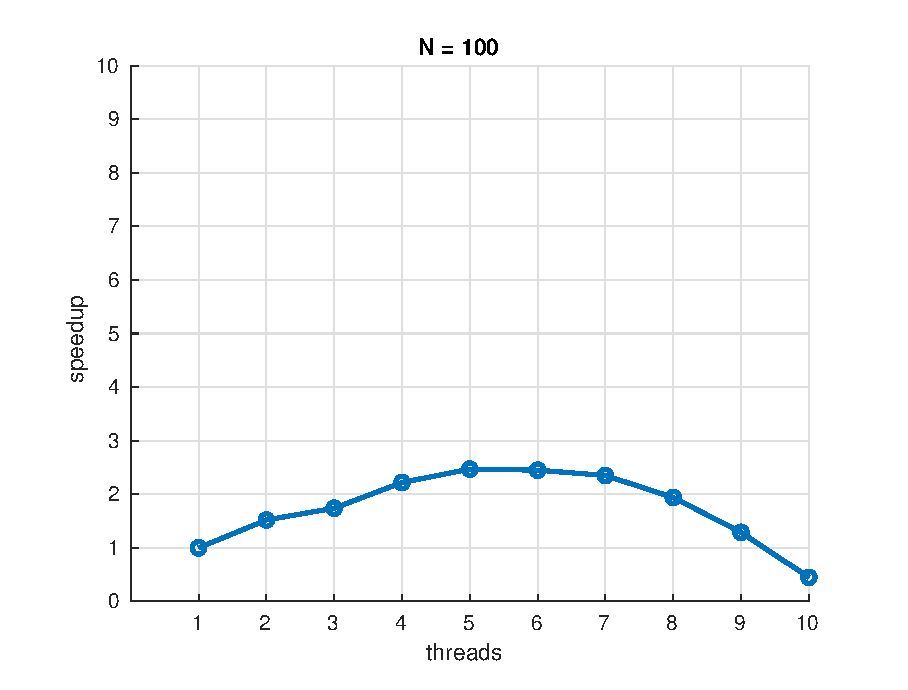
\includegraphics[width=3.2in]{../Paper/fig/speedup100.eps}
\end{figure}

\end{frame}


\begin{frame}{N = 1000}

\begin{figure}[H]
\centering
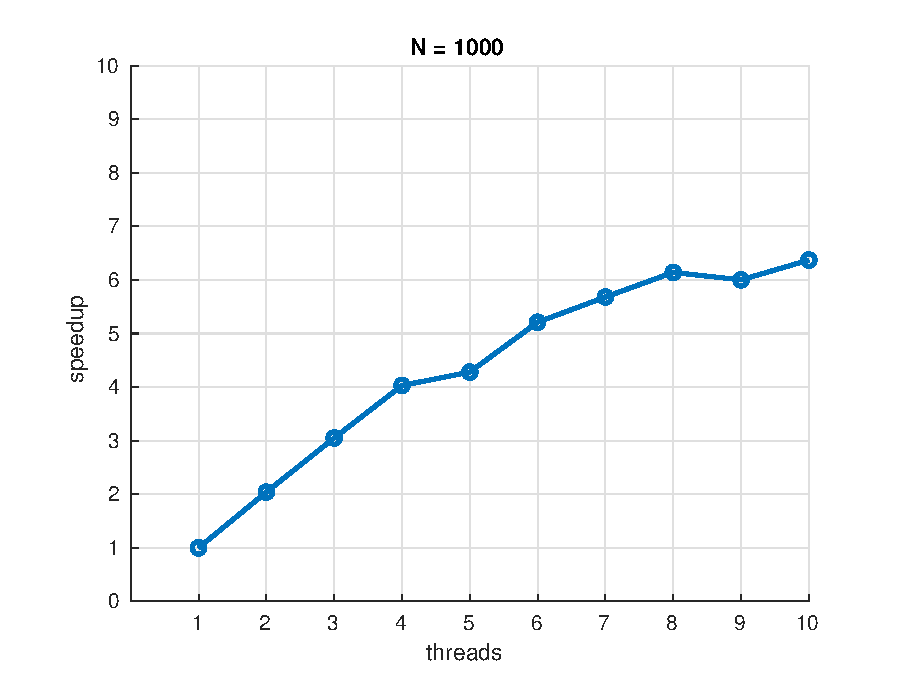
\includegraphics[width=3.2in]{../Paper/fig/speedup1000.eps}
\end{figure}

\end{frame}


\begin{frame}{N = 10000}

\begin{figure}[H]
\centering
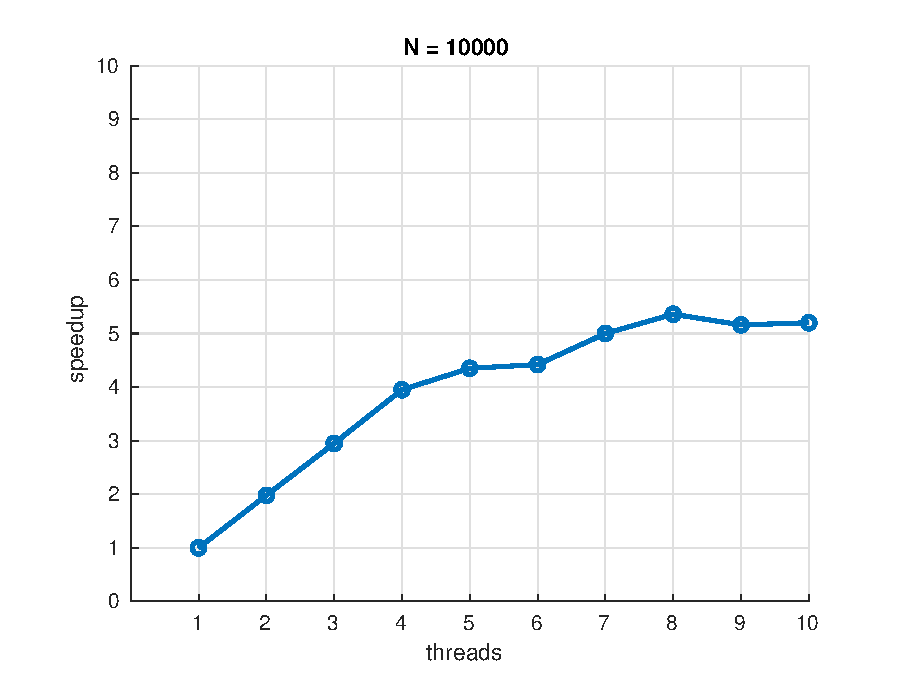
\includegraphics[width=3.2in]{../Paper/fig/speedup10000.eps}
\end{figure}

\end{frame}


\begin{frame}{N = 20000}

\begin{figure}[H]
\centering
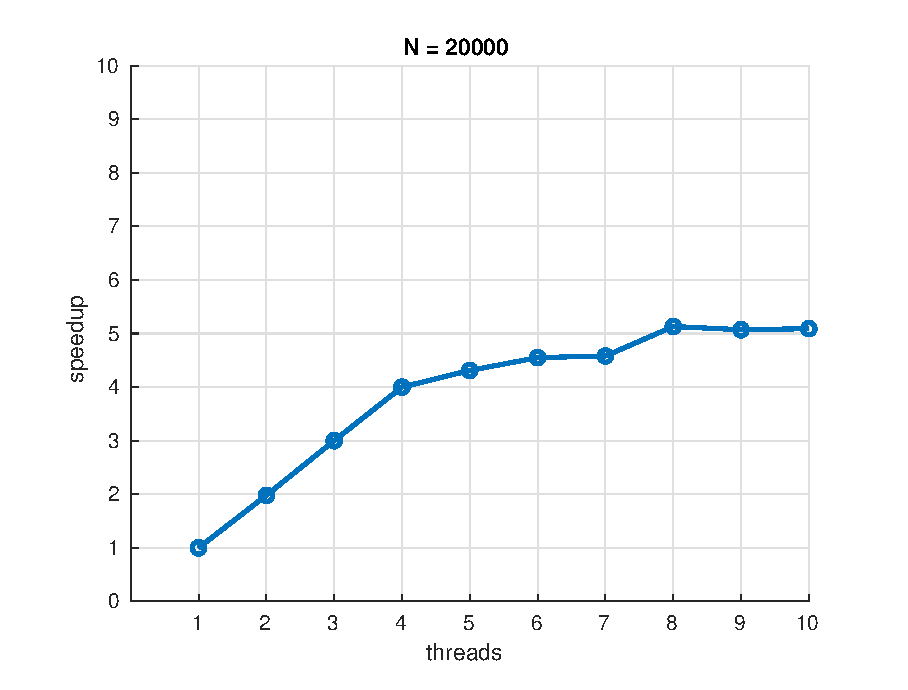
\includegraphics[width=3.2in]{../Paper/fig/speedup20000.eps}
\end{figure}

\end{frame}


\begin{frame}{N = 50000}

\begin{figure}[H]
\centering
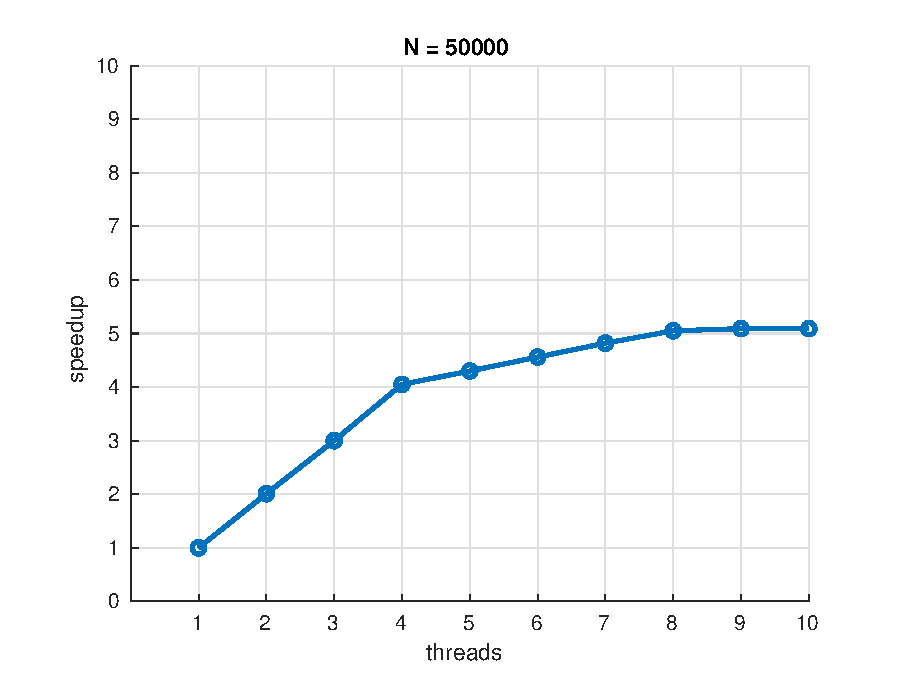
\includegraphics[width=3.2in]{../Paper/fig/speedup50000.eps}
\end{figure}

\end{frame}


\begin{frame}{Speedup growth}
The speedup growths with three different patters due to the \textit{hyper-threading} technology.

\begin{figure}[H]
\centering
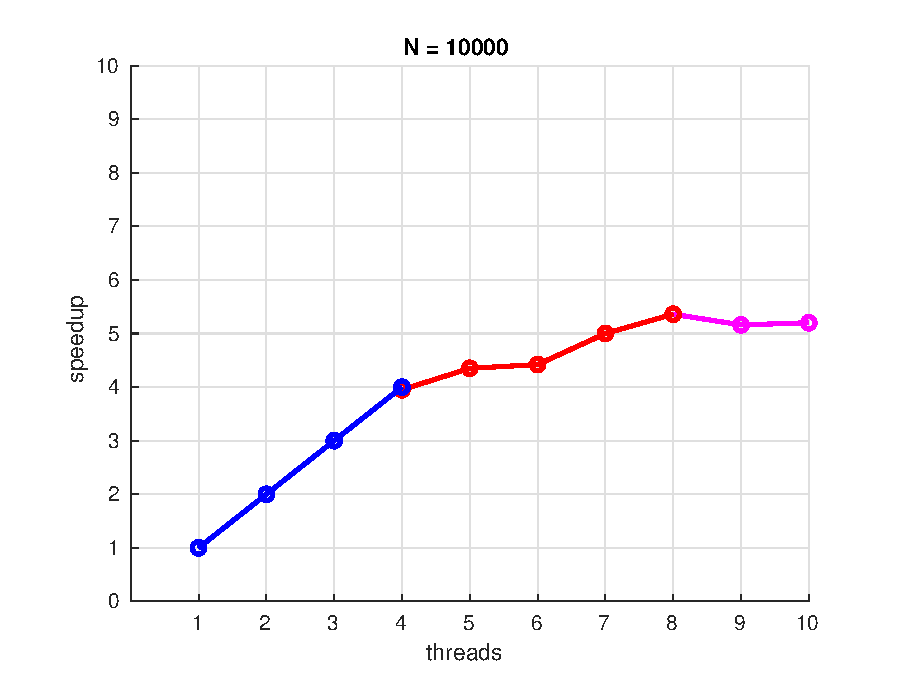
\includegraphics[width=3.2in]{../Paper/fig/speedup10000Colors.eps}
\end{figure}
\end{frame}


\begin{frame}{$\sigma$ = 1}

\begin{figure}[H]
\centering
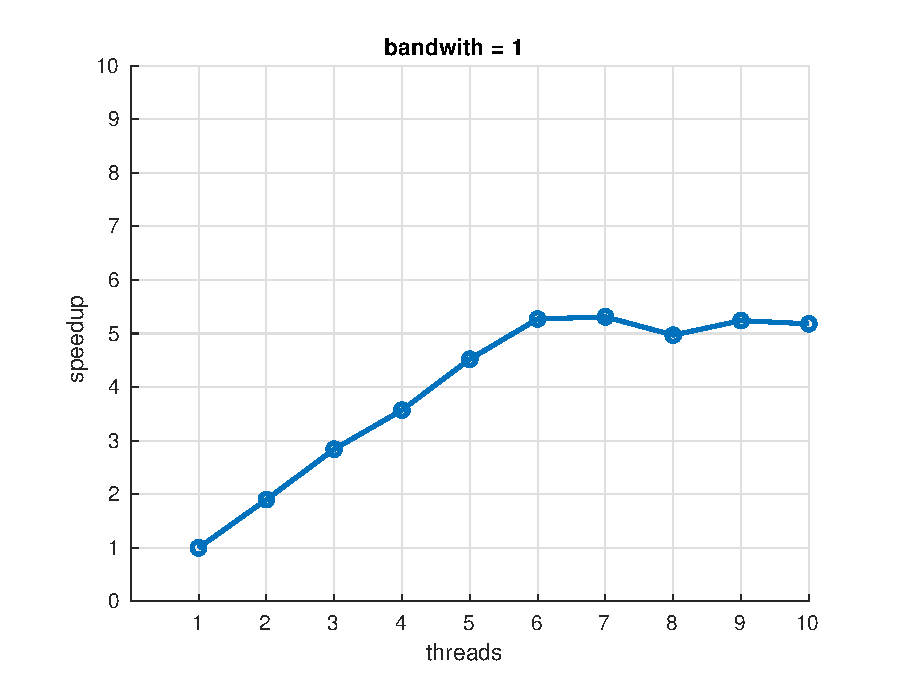
\includegraphics[width=3.2in]{../Paper/fig/speedup1b.eps}
\end{figure}

\end{frame}


\begin{frame}{$\sigma$ = 2}

\begin{figure}[H]
\centering
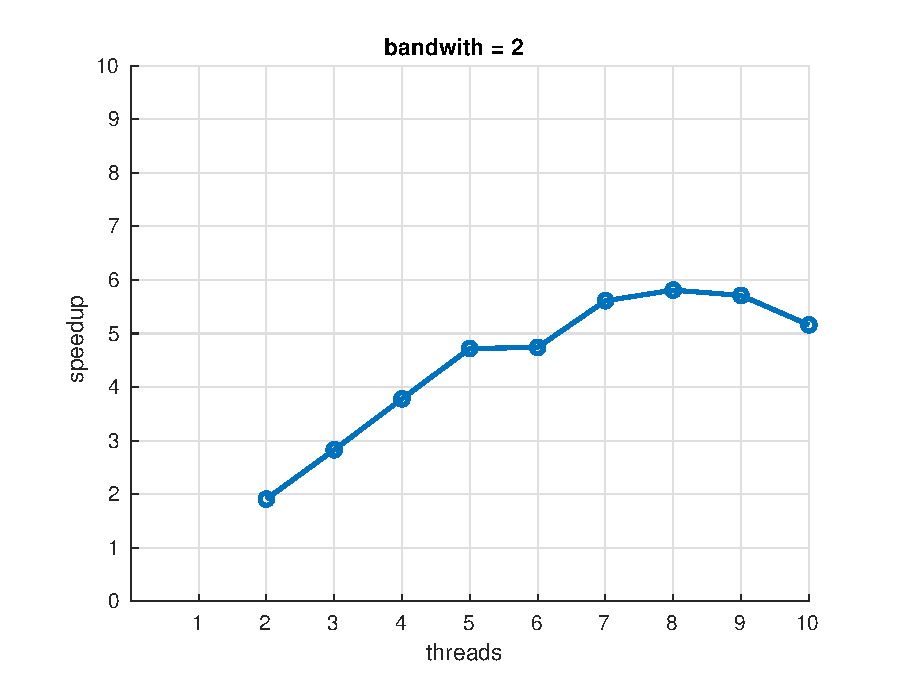
\includegraphics[width=3.2in]{../Paper/fig/speedup2b.eps}
\end{figure}

\end{frame}


\begin{frame}{$\sigma$ = 10}

\begin{figure}[H]
\centering
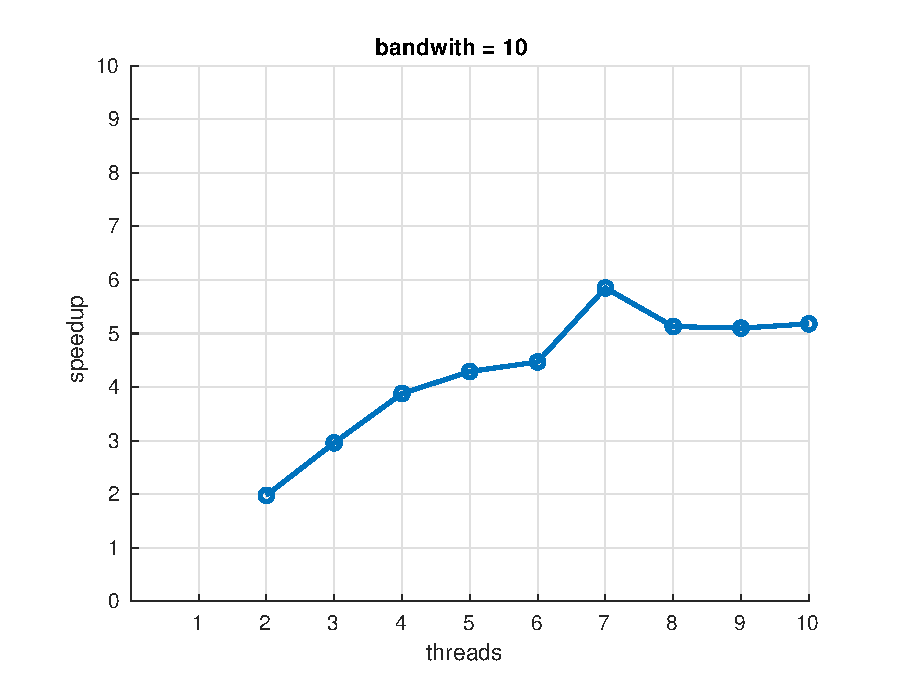
\includegraphics[width=3.2in]{../Paper/fig/speedup10b.eps}
\end{figure}

\end{frame}

\begin{frame}{Bandwith influence on the speedup}
The growing trends from one to four cores seem to be almost all the same for every value of the bandwith parameter. So we can conclude that if the dataset is big enough, the choice of the bandwith parameter will not influence the speedup.
\end{frame}


\end{document}
